\documentclass{article}

% Compilation and document writing packages
\usepackage[toc,page]{appendix}
\usepackage[british]{babel}
\usepackage[style=ieee,backend=bibtex]{biblatex}

% Formatting packages
\usepackage{fancyhdr}
\usepackage[margin=2cm]{geometry}
\usepackage[ddmmyyyy]{datetime}
\usepackage{url}
\usepackage[tight]{shorttoc}
\usepackage{tabulary}

% List packages
\usepackage{enumitem}

% Figure packages
\usepackage{graphicx}
\usepackage{float}
\usepackage{subcaption}

% Helpful packages
\usepackage{pdfpages}
\usepackage[color=yellow]{todonotes}
\usepackage{color}

\bibliography{refs}

\newif\iffinal
\newcommand{\ID}{CP-CBU-155 }
\newcommand{\IMAGEPATH}{../Images/}
\newcommand{\red}[1] {
	\iffinal
	\else
		\color{red}
		#1
		\color{black}
	\fi
}
\newcommand{\todomessage}[1] {
	\iffinal
	\else
		\todo[inline]{#1}
	\fi
}

%\finaltrue
\finalfalse

%opening
\title{Capstone Project
	  \vfill
	Final Report
	\vfill
	2015}
\author{}
\date{}


\begin{document}
	
\begin{titlepage}
	\begin{figure}
		\centering
		\includegraphics[width=100pt]{\IMAGEPATH emblem}
		\label{fig:emblem}
	\end{figure}
\end{titlepage}

\maketitle

\begin{tabular}{ll}
	Project Title: & Hybrid UAV Development for Emergency Response \\ 
	\\
	Date: & \date{\today} \\ 
\end{tabular}
\\
\\

\textbf{\textit{Project Team Information}}
\\
\\

\begin{tabular}{ll}
	Identifier: & \textbf{\ID} \\\\
	Student workers: & \begin{tabular}[t]{@{}ll}
		Matthew De Bono & 390758 \\ 
		Alexander Daraio & 389844 \\ 
		Wesley Lim & 391053 \\ 
		Shanon Loveridge & 218041 \\ 
	\end{tabular}  \\\\
	Academic supervisor: & Colin Burvill \\\\ 
	Academic examiner: & Saman Halgamuge\\\\
	Industry Mentor: & Jonathon Manton, DEEE\\\\
	Version: & 1.0 \\\\
\end{tabular} 

\vfill
\vfill

\newpage

\section*{Acknowledgments}
Team \ID would like to make the following acknowledgments:
\begin{itemize}
	\item \textbf{Shanon Loveridge}: for his commitment and contributions to the project throughout the year.
	\item \textbf{Dr Colin Burvill and Dr Saman Halgamuge}: for guiding and supporting us throughout the year.
	\item \textbf{Andrew Nolan and Jeffrey Hollingworth}: for their expertise, advice and generous equipment loans.
	\item \textbf{Phoenix Multicoptor teams}: for the laughs, advice and co-operation throughout the year.
	\item \textbf{Melbourne School of Engineering}: for workspace to complete our project.
\end{itemize}

\todomessage{Make sure to uncomment line here to generate Table of Contents, then comment out again}
\tableofcontents

\begingroup

% Modify ToC item separation
\makeatletter
\renewcommand\@dotsep{10000}
\patchcmd{\l@section}{%
	\addvspace{1.0em \@plus\p@}% original code line
}{%
	\addvspace{0.5em \@plus 0.3\p@}% substitute code line
}{}{}
\makeatother

% Generate ToC in document
%\shorttoc{Contents}{2}
\endgroup

\newpage

\section{Executive Summary}
The Executive Summary offers a succinct statement of your findings and contributions.

It will summarise the project description and your contributions to the associated discipline.  

This section can be based on key sentences and paragraphs from your Scope of Works and Progress Report documents, and your Conclusions and Recommendations section.

No more than five pages of text and images.


\newpage

\section{Introduction}
\subsection{Context}
\todo[inline]{Get references}
Drones, or UAVs, are not new technologies. UAVs are currently used extensively, for both offensive and defensive operations, by militaries across the globe. There is also a strong push for UAVs in commercial applications, such as package delivery and crop monitoring, and an ever-growing population of hobbyists, adventurers and athletes using drone-mounted cameras to capture everything from weddings to skiing down mountains.\\

\todo[inline]{Add more negatives/problems}
However, there are several applications that are infeasible for current drone technology. Rotor-based aircraft like the DJI Phantom (Figure \ref{fig:lidar}) are highly maneuverable, easy to control, and can be launched from almost any location, but as a result of their large power demands have very limited range/endurance. This makes them difficult to use in applications requiring long distance travel, such as package delivery.

\begin{figure}[!h]
	\centering
	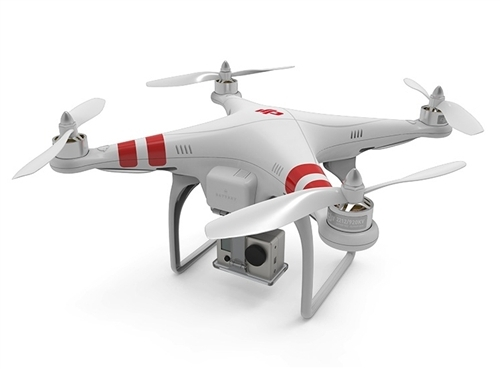
\includegraphics[width=150pt]{\IMAGEPATH /Aircraft/djiPhantom}
	\caption{DJI Phantom, a commercially available UAV}
	\label{fig:dji}
\end{figure}

\todo[inline]{Add more negatives/problems}
Wing-based aircraft such as those based on the Skywalker X8 frame (Figure \ref{fig:x8}) can achieve much greater travel distances as a result of higher efficiency flight. However, winged aircraft require open spaces to land safely, making them difficult to use in cramped or obstacle-rich applications such as low-altitude search near cities or forests.

\begin{figure}[!h]
	\centering
	
\includegraphics[width=160pt]{\IMAGEPATH /Aircraft/x8}
	\caption{Skywalker X8 airframe, a common hobby starter}
	\label{fig:x8}
\end{figure}
 
The UAV Challenge is a competition organised by the Queensland University of Technology and the CSIRO. It is held every 2 years, and aims to push the boundaries of current autonomous aircraft technology. The 2016 challenge is titled ``Medical Express'', and seeks to overcome some of the issues raised above. The objectives of the 2016 Challenge are to use unmanned aircraft to assist in a medical emergency.\\

Competitors must develop an aircraft than can fly to a known location (up to 30km) through specific transit corridors, search for and correctly identify ``Outback Joe'', land close to him to accept a pre-prepared blood sample, and then fly back to base. All of these actions must be completed within an hour, and must be autonomous; that is, after receiving the ``start'' signal the aircraft must have no human input.\\

\todo[inline]{Not sure if this section fits in intro}
The time period of the competition extends from registration (before 2nd September, 2015) to final competition (week starting 19th of September, 2016), spanning over 1 year. Table \ref{tab:challenge} highlights the key dates and corresponding stages of the UAV Challenge.\\

\todo[inline]{Add completed to D1 once we get the response}
\begin{table}[!ht]
	\caption{UAV Challenge Timeline}
	\label{tab:challenge}
	\centering
	\begin{tabular}{ | l | l | }
		\hline
		\textbf{Events} & \textbf{Date} \\ \hline \hline
		Registration and Deliverable 1: Short Technical Report & 2nd September 2015 \\ \hline
		Deliverable 2: Technical Report and Video & 13th April 2016 \\ \hline
		Deliverable 3: Autonomous Flight Record & 3rd August 2016 \\ \hline
		Final ``Go/No-Go'' decision for teams & 10th August 2016 \\ \hline
		Medical Express Challenge & Week starting 19th September 2016 \\
		\hline
	\end{tabular}
\end{table}

\subsection{\ID Contributions}
This project involves the development of an autonomous Unmanned Aerial Vehicle (UAV) with the capabilities to compete in the 2016 UAV Challenge. From the task specified above, \ID have identified a number of design and performance requirements necessary for an aircraft to be successful in the Challenge:
\begin{enumerate}[label=\bfseries R\arabic*:] \itemsep-2pt
	\item Capacity to switch between automated and manual flight modes through user commands
	\item Payload receipt and transportation back to base
	\item Take-off and landing in obstacle-rich environments (i.e. without runway)
	\item Total flight travel distance of at least 60km
	\item Total flight duration of at least 60 minutes
	\item Automated in-flight identification of a target
\end{enumerate}

\todo[inline]{Might remove some of these in final}
Given the requirements and the timeline of the Challenge above, \ID sought to develop a working prototype with which to enter the 2016 UAV Challenge. As such, the following objectives were selected for the project:
\begin{enumerate}[label=\bfseries O\arabic*:] \itemsep-2pt
	\item Register for the 2016 UAV Challenge
	\item Provide a Bill of Materials for UAV development
	\item Development of a novel hybrid flight system, incorporating both Vertical Take-Off and Landing (VTOL) and Fixed-Wing flight modes, to achieve \textbf{R3}, \textbf{R4} and \textbf{R5}
	\item Development, documentation and implementation of autonomous flight controls
	\item Development of a low-cost, medium-range sensor system to enable object detection and path planning
	\item Development of in-flight search and obstacle avoidance mechanisms to achieve \textbf{R6}
	\item Establish a strong foundation for Capstone student teams to continue work in 2016
\end{enumerate}

The remaining sections of the report will discuss the work conducted by \ID in developing a working prototype for the UAV Challenge, beginning with formulating design requirements and constraints from the UAV Challenge specification. The following sections will discuss the various domains of the aircraft, including design, flight and planning systems, and sensing systems, with a particular focus on the novel transition system for hybrid flight. The report will end with conclusions and recommendations for future work.

\section{Literature Review}
\subsection{Mission Breakdown}
\label{sec:flightmaneuvers}
The Medical Express mission can be broken down into three discrete flight maneuvers:
\begin{enumerate}[label=\bfseries M\arabic*:] \itemsep-2pt
	\item Hover flight, including vertical take-off to cruising height, and landing
	\item Fixed-wing flight, navigating through waypoints and keeping within GeoFence boundaries
	\item Aerial search
\end{enumerate}

Using these maneuvers, completing the mission can be described as completing the sequence of actions\\
\begin{tabular}{r l l}
	1. & Mission start after being armed & (\textbf{M1}) \\ 
	2. & Navigate to Joe's location & (\textbf{M2}) \\ 
	3. & Aerial search to identify Joe & (\textbf{M3}) \\ 
	4. & Land near Joe to collect blood & (\textbf{M1}) \\ 
	5. & Take-off after being re-armed & (\textbf{M1}) \\ 
	6. & Navigate back to base & (\textbf{M2}) \\ 
	7. & Land at base & (\textbf{M1}) \\ 
\end{tabular}\\

Executing this mission on a purely fixed-wing or rotor-based aircraft is unlikely to be successful; instead, teams will need to design an aircraft that makes use of both flight modes. Analysis of the 2014 design, a purely fixed-wing aircraft, showed that converting it to a hybrid aircraft would not result in a suitable design for the Challenge. Given the aircraft's weight, adding the necessary equipment would add over 5kg, cost over \$500, and would result in less than 60 seconds of flight time. It was therefore decided the 2014 model would not be suitable for the 2016 competition; a detailed analysis can be found in Appendix \ref{sec:lastYear}.\\

As this project involves the development of a novel aircraft platform, there is a lack of academic literature that is relevant to the problem at hand. This review will instead collate examples of commercial and hobby systems that were used to inspire and guide the development of the aircraft.\\

\subsection{Aircraft Design}
\subsubsection*{Arcturus Jump}
The Arcturus Jump\cite{ref:arcturus} (Figure \ref{fig:arcturus}) is a quad-copter/fixed-wing hybrid, with propellers mounted across the wings for VTOL, and a propeller at the front for fixed-wing flight. Modifying an existing airframe to emulate this design would be straightforward, but the addition of the support structure for VTOL flight would add significant weight to the aircraft, decreasing thrust and maneuverability, and increasing drag. These factors make an aircraft of this design unlikely to achieve \textbf{R4} (60km endurance) and \textbf{R5} (60min of flight) of the UAV Challenge.

\begin{figure}[!h]
	\centering
	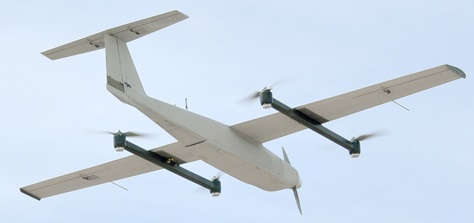
\includegraphics[width=150pt]{\IMAGEPATH /Aircraft/arcturus}
	\caption{Arcturus Jump 20}
	\label{fig:arcturus}
\end{figure}

\subsubsection*{X PlusOne}
The X PlusOne\cite{ref:xplusone} (Figure \ref{fig:xplusone}) is an incredibly fast and efficient hybrid with four front-facing propellers. It is extremely small and light, and would be relatively cheap to build, but is too small to replicate with an existing airframe. However, based on the activities of the 2014 UAV team, designing a completely new airframe would take a significant amount of time, and is not advised for this project.

\begin{figure}[!ht]
	\centering
	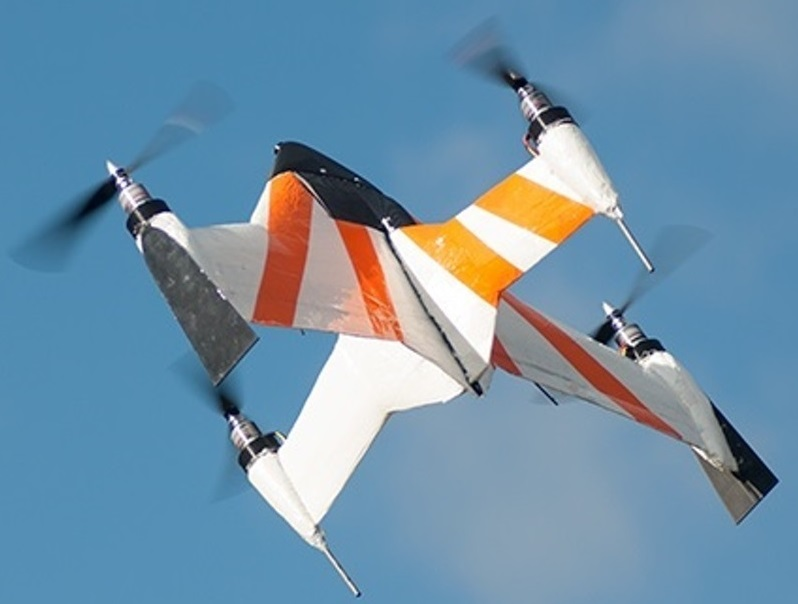
\includegraphics[width=120pt]{\IMAGEPATH /Aircraft/xplusone}
	\caption{X PlusOne}
	\label{fig:xplusone}
\end{figure}

\subsubsection*{TBS Caipirinha}
The TBS Caipirinha\cite{ref:caipirinha} (Figure \ref{fig:caipirinha}) is traditionally a hobbyist fixed-wing aircraft kit. However, several examples have shown it is possible to modify the Caipirinha to be a VTOL aircraft\cite{ref:caipirinhaVTOL} (Figure \ref{fig:caipirinhaVTOL}), with two front-facing propellers. Modifying the Caipirinha for hybrid flight would require minimal modifications to the airframe but would require the development of advanced control systems to alternate between VTOL and fixed-wing modes.

\begin{figure}[!ht]
	\centering
	\begin{minipage}{.5\textwidth}
		\centering
		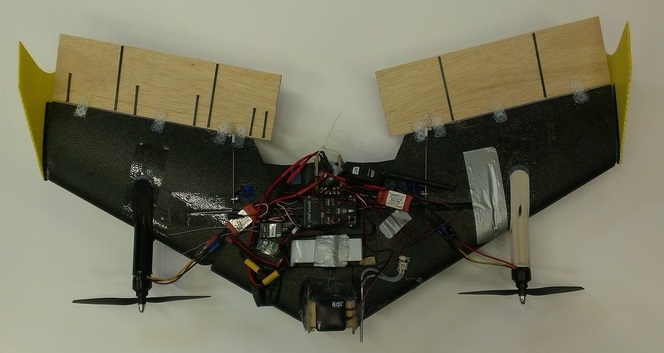
\includegraphics[width=135pt]{\IMAGEPATH /Aircraft/caipirinha}
		\caption{TBS Caipirinha}
		\label{fig:caipirinha}
	\end{minipage}%
	\begin{minipage}{.5\textwidth}
		\centering
		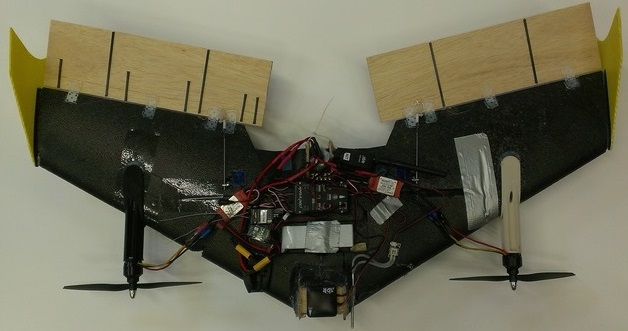
\includegraphics[width=155pt]{\IMAGEPATH /Aircraft/caipirinhaVTOL}
		\caption{Caipirinha modified for VTOL flight}
		\label{fig:caipirinhaVTOL}
	\end{minipage}
\end{figure}

\subsubsection*{Aerosense AS-DT01-E}
The Aerosense AS-DT01-E\cite{ref:sony} (Figure \ref{fig:sony}) is an autonomous hybrid VTOL/fixed-wing aircraft being developed by Sony Mobile in partnership with Japanese company ZMP. While the prototype aircraft would be an ideal candidate for the Challenge, as with the X PlusOne the design and construction of the airframe would be time consuming, and is not advised for this project.

\begin{figure}[!ht]
	\centering
	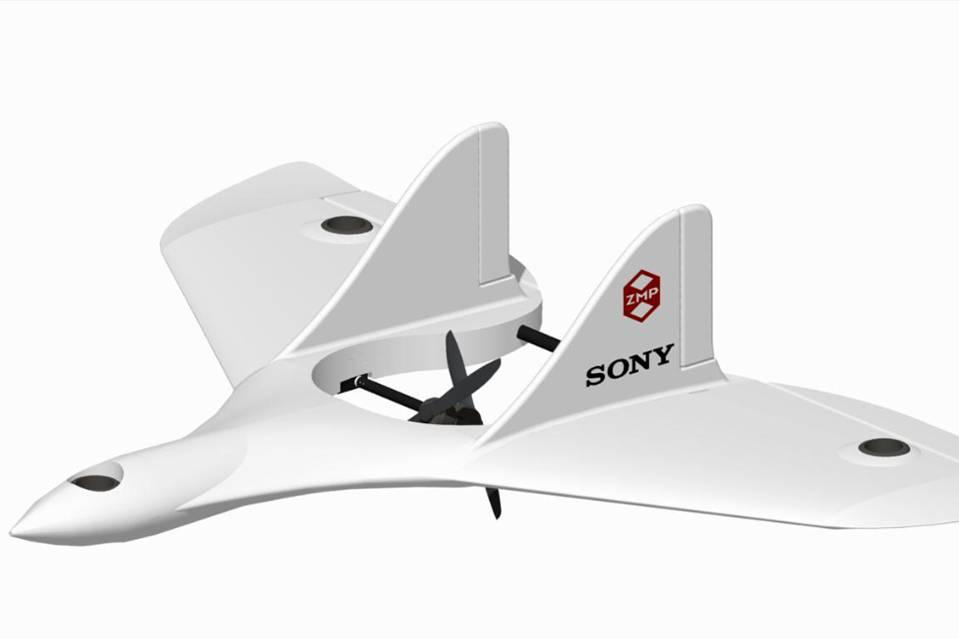
\includegraphics[width=160pt]{\IMAGEPATH /Aircraft/sony}
	\caption{Sony Aerosense}
	\label{fig:sony}
\end{figure}

\subsubsection*{FireFLY6}
Finally, the FireFLY6\cite{ref:firefly6} (Figure \ref{fig:firefly6}) is a remote control hybrid VTOL/fixed-wing aircraft consisting of six propellers arranged in 3 sets of two (Y6 configuration). This design can achieve 20-30 minutes of flight time, seven minutes of hover, and a cruising speed of 54km/h, and would be a strong contender in the UAV Challenge.

\begin{figure}[!h]
	\centering
	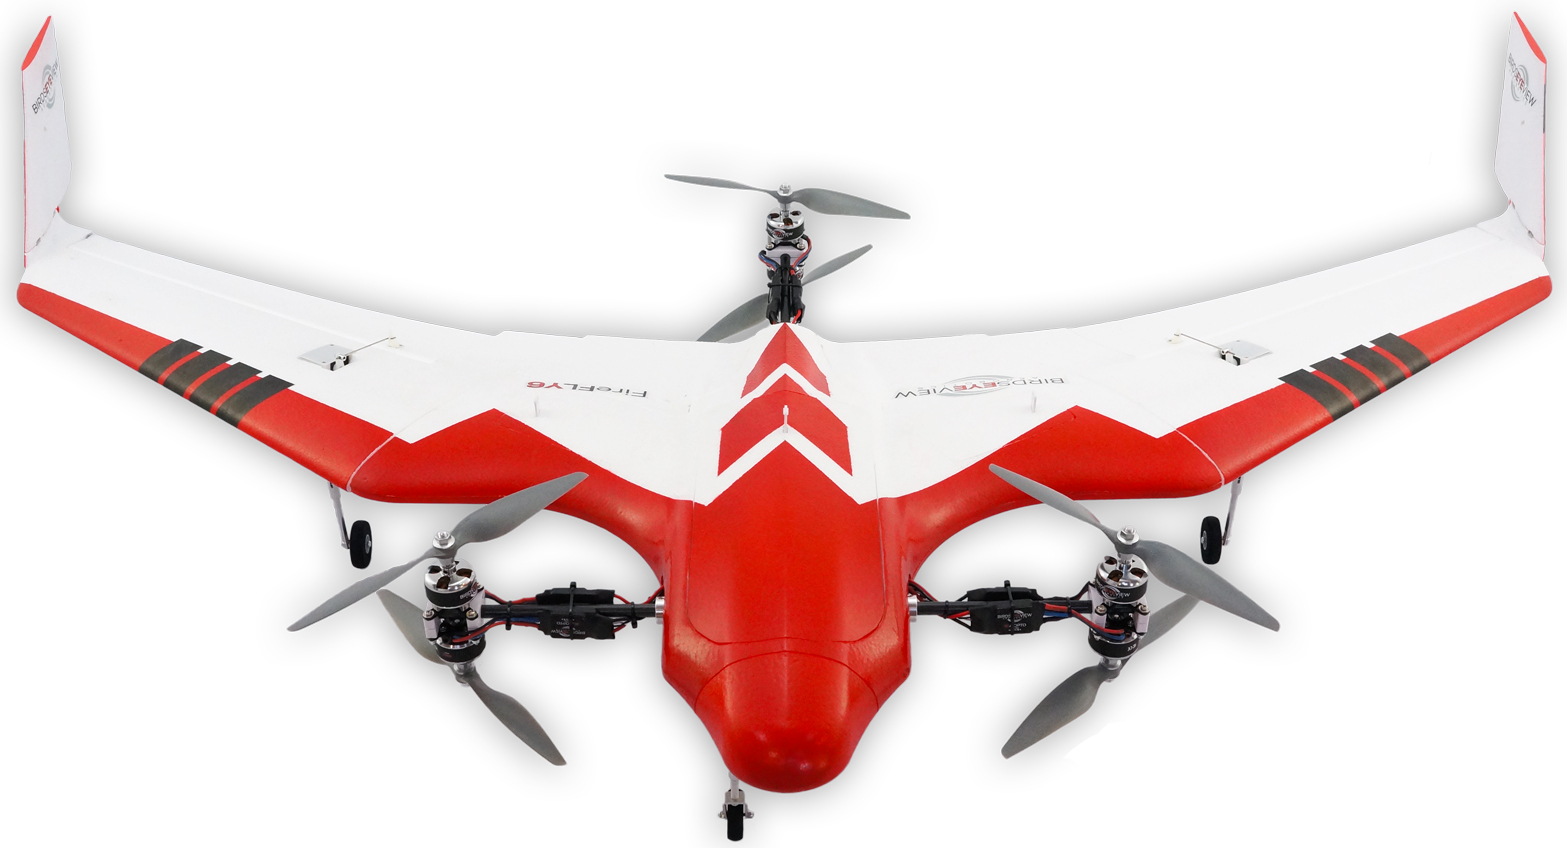
\includegraphics[width=160pt]{\IMAGEPATH /Aircraft/firefly6}
	\caption{FireFLY6}
	\label{fig:firefly6}
\end{figure}

\section{Aircraft Design}
\red{\begin{itemize}

\item Extra stuff... legs, new gears, glued on parts and changed placements for wings(Alex))



\end{itemize}}

\red{Some of these sections are already in the lit review, like the decision on flight controller}
\subsection{Basic Configuration}
The specifications for parts to fit the design were first modeled using eCalc\cite{ref:ecalc}, a website for calculating the performance of aerial vehicles, a commonly used tool in the drone building community. This site has a vast collection of empirical data for motors, propellers, batteries and configurations and boasts an accuracy of $\pm$10\% for all calculations. Details of the modeling can be found in Appendix \ref{sec:ecalc}.

\subsubsection*{Configuration}
To achieve the novel transition system sought after from the start of the project, the optimal motor configuration was investigated for the job. It was realized that a selection of the motors would need to be capable of being rotated forward to support the transition function and for such a purpose a `tri-copter' formation was selected.\\
		
A Y-3 configuration was selected over a Y-6 configuration, as it would lead to a lighter and cheaper aircraft. However, the aircraft was designed to be capable of being 'upgraded' to a Y-6 configuration if the need arose. The three motors would provide lift in VTOL mode, the front two motors being mounted vertically utilizing a mounting system capable of being rotated forwards $90^{\circ}$ to facilitate the transition system and fixed-wing flight. The rear motor mount system was designed to be tilted laterally through the use of a servo-motor to enable the yaw mechanism of the aircraft.\\

\subsubsection*{Airframe}
In order to begin design and development on critical subsystems, a pre-designed `off the shelf' airframe was desired; for this purpose a Skywalker X-8 Flying Wing was selected as it offered a large amount of under canopy storage room, the greatest wingspan to weight ratio of the airframes investigated, fast low power cruise speeds, was stated to be capable of carrying a maximum all-up-weight (AUW) of greater than 3.5kg, was well priced, well reviewed and available quickly from Australian suppliers. Being made out of foam also made it wasy to modify into the required hybrid frame.
		
		
\subsubsection*{Carbon Fiber Poles and Supports}
SThe hybrid frame was created using a combination of two 12mm carbon fibre poles (front and back) and 3D printed mounts and supports. As gear systems, mounts and legs needed to be attactched, all holes in the rod due to fastening were drilled parallel to the base of the drone in order to minimise any reductions in strength (as the top and bottom of the poles have tesnsile and compressive stresses when hovering).
	
\subsubsection*{Motor}
The motors chosen needed to efficiently hover, but at the same time be able to cruise in fixed wing mode using minimal battery power. As such, the Turnigy SK3 3542 800kv motors were chosen. They are efficient, well priced, well reviewed and very effective at completing both objectives. They were also the motors used by \red{[CITE VID]} to achieve long range flight.
	
\subsubsection*{Propellers}
Modelling using eCalc suggested that smaller propellers provide better performance in fixed wing flight (less drag, weight), but larger propellers are better suited for VTOL (more thrust), with modelling presented in \red{[ADD APEN]}. As such, two sets of propellers were purchased (11$\times$5.5 and 12$\times$6) in both plastic and carbon fiber.
	
\subsubsection*{Servos}
A servo at the front of the plane, that rotates the front pole was chosen as the best option for the transition system. A servo was also required at the back of the plane to rotate the back shaft for yaw. Both servos chosen were Turnigy TGY-4409MDs, capable of 8.65kg.cm of torque at 5v, which has shown to be more than enough. 
		
\subsubsection*{Battery}
The primary concern for maximising flight time/range is by reducing weight. Multistar 8000 mAh batteries were selected as they allow for a much higher capacity at a lighter weight than conventional LiPo batteries. For flight testing the current protoype, two in parallel are being used. 
	
\subsubsection*{Flight Controller}
Following the discussion presented in \cite{ref:controller_comparison}, the PixHawk flight controller was found to be more powerful and faster, and more importantly, easier to reconfigure and add software to.

\subsection{Hardware Architecture}
\red{Basically how we intend to meet every requirement for the challenge. Put in circuit diagrams here, archetecture, information regarding long range network transmitters, and basic intro to sensors, automation and transition. Basically introducing what the overall plan looks like and what we have covered from that. Maybe do a chart or table or something.}

\subsection{3D Printing}
In order to enable proper stable and robust mounting of all motors and mounting systems, custom prototyping using 3D printed parts and iterative design was utilized to fit within the X-8 frame. The major components of design were split up into the `Motor Mounts', the `Front  Mounting System' and the `Back Mounting System'.\\

The Motor Mounts were designed to secure each motor to it's corresponding mounting pole, and while the basic design was straight forward, a couple of design iterations were required in order to come up with a truly robust design. Cylindrical inserts (also 3D printed) were utilized in order to prevent the crushing of the carbon fiber rod in the event of over tighening the fasteners and a hose clamp was used to ensure an equally distributed squeezing force was applied from the mount to the pole.\\

The Front Mounting System was designed to incorporate the transition system, while also being stable enough to withstand disturbances associated with being placed at the front of the aircraft.
The Back Mounting System needed to incorporate the yaw servo-motor system. The direction in which a design is 3D printed plays a vital role in where its strength and weaknesses lie. Each print was orientated to maximise the strength of the layers against the most likely mode of failure from the forces and moments being applied.\\

In order to achieve a ``true'' circle shape and thus lower friction for mated parts, critical ring shapes in designs were replaced by flatly printed ring inserts. These ring inserts were then either press fit into other printed components or ``merged'' onto other printed components using acetone. See Table \red{[REF]} for all 3D printed parts, iterations and settings.  \red{[WILL MAKE TABLE SOON]}.

\subsection{Calibration}
\subsubsection*{Motor and Propeller Balancing}
In order to eliminate vibrations generated from propellers they must be balanced, which is accomplished by either adding (using tape, or similar) or removing (shaving off material) mass from either side of a propeller. A non-destructive method was preferred, so small pieces of tape were added to the propellers using the balancing apparatus shown in figure \red{[ADD FIGURE]} to ensure the mass distribution was equal.  Seismograph testing (using a free app) of the propellers before and after balancing showed a very obvious decrease in vibrations. Based on this app, we were also able to determine that motor vibrations were negligible comparitively.\\

\subsubsection*{Mass Balancing}
The center of gravity (CoG) of the new aircraft may be changed by repositioning the batteries (the heaviest items to be carried). The CoG needed to meet two specifications:
	\\\\The center of mass had to be at the center of thrust of the VTOL. As there are two propellers in the front and one in the back this would be one third of the distance from the front propellers to the back propeller (approximately 30cm from the front motors), resulting in an equal moment about the center of gravity. This would allow all motors to produce the same amount of thrust without causing the aircraft to tilt.
	\\\\The centre of mass also had to be at the centre of lift, which for Skywalker X-8 is given as 44cm from the nose of the aircraft. The distance of the front motors from the nose of the aircraft is approximately 14cm. With the center of mass positioned 30cm from the front motors, the center mass and center of lift are coincident.\red{[VALIDATION FROM CALCULATIONS]}
	
\subsubsection*{ESC Calibration}
The receiver and pixhawk signal were calibrated into the electronic speed controllers (ESCs) by setting a minimum and maximum motor throttle. This was done by programming the ESCs simultaneuously using the manufacturors manual.

\subsubsection*{Pixhawk Calibration}
The inbuilt compass and accelerometer of the pixhawk required tuning each time the internal configuration of the drone changed in order to ensure level flight. This is achieved through setting points in the open source program, Mission Planner. A once off power module voltage and radio calibration were also required, to ensure correct battery monitoring, and input. 

\subsubsection*{PID Tuning}
The Pixhawk comes with in built PID paramaters ready to be modified for all required control applications.  There are many ways to tune the Pixhawk PIDs. For the drone, basic tuning was first performed by setting the roll, pitch, and throttle gains and sensitivities to ensure stable and responsive flight controls. Then as recommended by the platform, an auto-tune was then completed and implimented on the craft to ensure the best possible PID values for the custom drone. This involved holding the drone in altitude hold mode while the drone tested responses and set the very best PID parameters. This was later verified by checking flight logs, see \red{[ADD LOG STUFF]}. When the wings were finally added, as the inertia, disturbances and weight of the plane changed, an auto-tune was required again see \red{[ADD LOG STUFF]}.




\section{Flight Validation}
\label{sec:flight}
\red{
\begin{itemize}
	\item Development of basic flight systems after construction of airframe
	\item Discuss Prototype \#1
	\item Testing of basic flight with Prototype
\end{itemize}}

\section{Transition}
\red{\begin{itemize}
\item more about software?
\item information pertaining to future test flights

\end{itemize}}


\subsection{Why Transition?}
In order to complete the objectives, long range flight would be required. This is why a transition system was necessary to implement, allowing the VTOL drone to fly forwards, both faster and more efficiently. This will hopefully allow the drone to fly for the required 1 hour flight time needed in deliverable 2, and allow it to travel for over 60 km that is required for the task. 

\subsection{Forward flight}
The plane was designed from the beginning to deal with transition. It was decided that two propellers of the VTOL copter would rotate forwards, creating a forward thrust and generating lift on the wings.  
\\\\
Firstly, a combination of wings and front motors capable of forward flight were required.  As mentioned the Skywalker X8 was shown to work well with forward flight, and the motors chosen (Turnigy SK3-3542-800) were the same chosen by others online, some who have achieved over 142km of flight time with the Skywalker(link?). eCalc (see Appendix \ref{sec:ecalc}, Figure \ref{fig:fixed}) suggested that at 3.5kg the aircraft had an estimated stall speed of 32km/h and a cruising speed of 82km/h with this combination. Additional calculations (see \ref{sec:stall}) further verified flight by ensuring a worst case stall speed at 4kg, with the Skywalker's minimum coefficient of lift for level flight at 0.5, of 45.5km/h. As the air will be forced over the wing, it is believed this should create further lift.

\subsection{Gyroscopic Forces}
An analysis of the gyroscopic forces acting on the motors during transition was performed to determine the required configuration of the motors, the strength of the shaft in between the two motors, and the torque required to make the transition. The calculations (see  \ref{sec:gyro}) showed that gyroscopic forces would create a moment perpendicular to the direction of rotation based on the direction of the motor angular velocity. To counteract this, two propellers on the front spinning in opposite directions would create zero net moment, and therefore the drone would be able to remain steady after transition. This was already the plan as counter rotating propellers also create a zero net angular momentum from the front in VTOL mode, making control much easier.\\

From this, the total moment created by this gyroscopic motion was 3.1Nm in the centre of the shaft, however for our rotation speed, this was less than the moment gravity exerted on the shaft while the motors were hovering, which was 9.156Nm. Lastly, the transition system would need to hold the propellers steady for any other gyroscopic forces. In particular if the aircraft rolls too fast, it would create a moment in the front. Due to the counter-rotating front motors however, these forces again would be opposite and counteracting.\\

The front servo would therefore receive no counter moment in flight. An arbitrary servo was chosen at 8.65kg/cm (0.85Nm), through testing it was found to behave satisfactorily against frictional or other unknown forces. This was verified by holding the drone down in tests and ensuring transition was possible at full motor speed.

\subsection{System Design}
For implementation a 1:1 gear system attached between the servo and motor shafts was installed (see Figure \ref{fig:gearsys}). This allowed for full rotation of the servo, and maximum accuracy.  Through testing of PWM values, it was set up to rotate by 90 degrees as required. A new mode was created through the open source Pixhawk firmware called “Fixed-Wing”, and possible transition from the VTOL modes was also set-up. This was created such that when a switch on the controller is turned, the front pole and motors rotate forwards 90 degrees, the VTOL control systems turn off, and the fixed wing control systems take over.\\

So far, a manual fixed wing mode has been created. It turns off VTOL control systems and changes the user input from controlling the rotation of the multi-copter, to the control surfaces of the aircraft when entering this mode. This meant programming such that pulling down or up on the left stick meant the flaps move up and down respectively for pitch, and moving the right stick moves the flaps in opposite direction for roll.  In order to implement this changes to the firmware were required.  This meant having  a complete understanding of the programming behind both the Pixhawk and the open source ardupilot project, and it also meant contributions were made to this open source platform. Eventually other modes would need to be created to complete the task, such as automated modes, or modes with basic stability control. \\
\todomessage{dev site references?}

\begin{figure}[!ht]
	\centering
	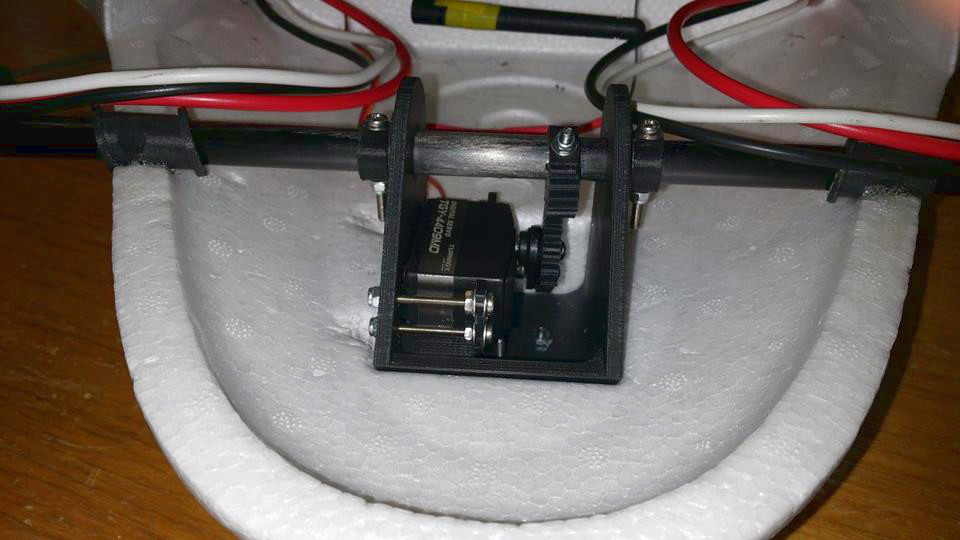
\includegraphics[width=300pt]{\IMAGEPATH /Prototype/gear_system}
	\caption{Front gear and mounting system}
	\label{fig:gearsys}
\end{figure}

\subsection{Testing}
A number of steps needed to be taken to transition into fixed wing mode: 
\todomessage{firefly instruction vid reference https://www.youtube.com/watch?v=VPUSLzj02dA}

\begin{itemize}
\item In altitude hold keep the throttle at 50\% and move the aircraft forwards to create some initial speed
\item At a stable but fast speed level the aircraft
\item Flick the transition switch 
\item Lower the throttle
\item Pull up and raise the throttle as required

Once the system were built, off-line tests were conducted by holding the aircraft down and rotating the front rotors while at hover speed. Control surfaces on the wings were also tested. 

\todomessage{actual transition results}
		
\end{itemize}


\section{Autonomous Flight}
\subsection{Breaking Down the Challenge}
\label{sec:flight}
Any aircraft participating in the UAV Challenge must be autonomous, only interacting with a human to be armed or disarmed at the beginning and end of the mission. In order to develop 
The Medical Express mission can be broken down into three discrete flight maneuvers:
\begin{enumerate}[label=\bfseries M\arabic*:] \itemsep-2pt
	\item Vertical take-off to cruising height, and landing
	\item Fixed-wing flight, navigating through waypoints and keeping within GeoFence boundaries
	\item Aerial search
\end{enumerate}

Using these maneuvers, completing the mission can be described as completing the sequence of actions\\
\begin{tabular}{r l l}
	1. & Mission start after being armed & (\textbf{M1}) \\ 
	2. & Navigate to Joe's location & (\textbf{M2}) \\ 
	3. & Aerial search to identify Joe & (\textbf{M3}) \\ 
	4. & Land near Joe to collect blood & (\textbf{M1}) \\ 
	5. & Take-off after being re-armed & (\textbf{M1}) \\ 
	6. & Navigate back to base & (\textbf{M2}) \\ 
	7. & Land at base & (\textbf{M1}) \\ 
\end{tabular} 

\subsection{Development}
Figure \ref{fig:softwarearchitecture} shows the autonomous flight and intelligence architecture implemented on the aircraft.

\red{Considerations:
	
	time cost -> prototype style / separate each module (allows cut off were we get to with some functionality)
	Extendibility -> for future years
	Concurrency -> Multiprocessing
	Latency -> processes polling / non blocking io etc
}

\red{Autonomy on Raspberry Pi}

\red{\begin{itemize}
	\item Generation of flight path, currently from text file but ideally based on sensing (flight.py)
	\item Capability for executing known/expected commands by sending to PixHawk (autopilot.py)
	\item Monitoring status of aircraft such as position, velocity (uavstate.py)
	\item Monitoring status of world such position of obstacles, waypoints (worldstate.py)
	\item Logging of flight conditions, sensing and motion (logging.py)
	\item Communicate with base station (interface.py)
\end{itemize}}

\begin{figure}[!ht]
	\centering
	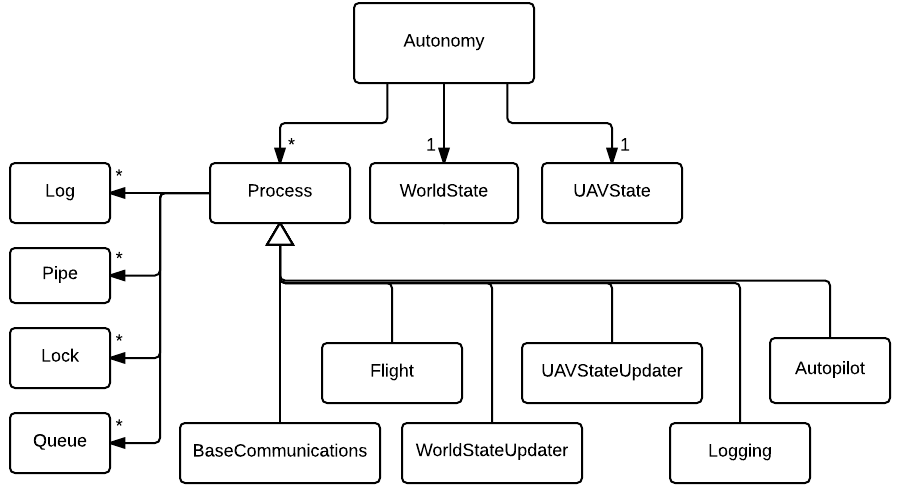
\includegraphics[width=350pt]{\IMAGEPATH /Diagrams/software}
	\caption{High level software architecture}
	\label{fig:softwarearchitecture}
\end{figure}

\begin{figure}[!ht]
	\centering
	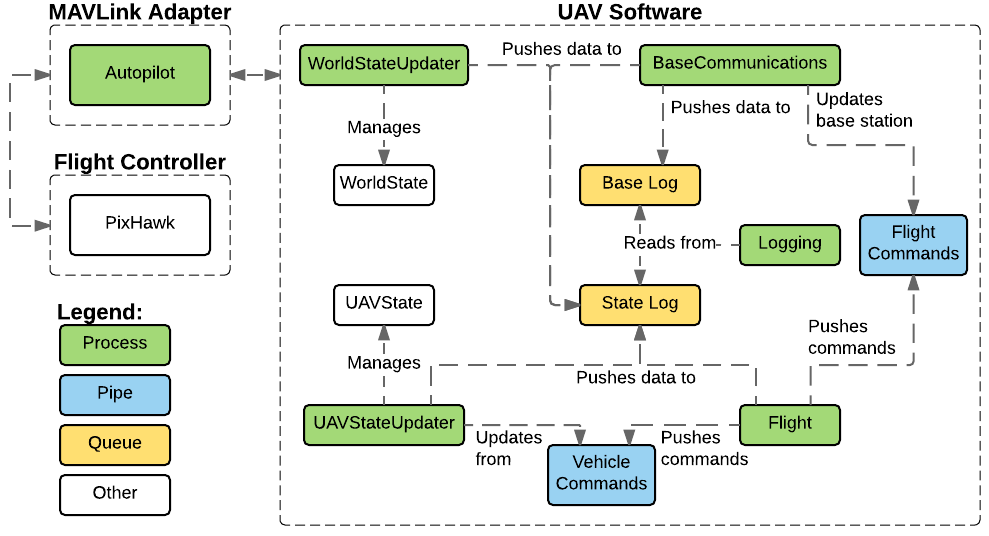
\includegraphics[width=350pt]{\IMAGEPATH /Diagrams/interaction}
	\caption{Interaction between software modules}
	\label{fig:softwareinteraction}
\end{figure}
\subsection{Testing}
\red{Software in the Loop}

\begin{figure}[!ht]
	\centering
	\includegraphics[width=200pt]{\IMAGEPATH emblem}
	\caption{Software in the Loop testing}
	\label{fig:sitl}
\end{figure}

\section{Sensing}
\label{sec:sensing}
Figure \ref{fig:sensing} outlines the on-board sensing capabilities that are available to the aircraft. The sections below detail the use of each sensor during a mission, and are separated according to the different stages of the UAV Challenge's mission, as introduced in Section \ref{sec:flight}. 

\begin{figure}[!ht]
	\centering
	\includegraphics[width=300pt]{\IMAGEPATH sensors}
	\caption{Onboard sensing capabilities for Prototype \#1}
	\label{fig:sensing}
\end{figure}

\subsection{All Stages}
\subsubsection*{Raspberry Pi}
The Raspberry Pi will act as the aircraft's on-board computing platform, providing autonomy by giving flight commands to the flight controller, as well as the processing and intelligence for path planning, and object detection. It will also pull flight data from the PixHawk and other sensors, and generate detailed flight logs for later review.

\subsubsection*{PixHawk Flight Controller}
The PixHawk will control the aircraft's flight functionality, such as controlling motors and ailerons, and executing flight paths and commands from the Raspberry Pi.

\subsection{Vertical Take-Off and Landing (M1)}
\subsubsection*{Ultrasonic Module}
The ultrasonic module will be mounted underneath the aircraft. The GPS and altimeter will provide altitude measurements during fixed-wing flight; the ultrasonic will augment these by providing a more reliable and controllable height measurement during rotor-based flight, assisting with search and landing.

\subsection{Fixed-Wing Flight (M2)}
\subsubsection*{PixHawk Sensors}
It also has several in-built or plug-and-play sensors, including a 3-axis accelerometer, altimeter, compass, and GPS. The PixHawk will provide the aircraft's telemetry to the Raspberry Pi and the base station, which will be augmented by the additional sensors below.

\subsection{Aerial Search (M3)}
\subsubsection*{Webcam}
The webcam will be mounted beneath the nose of the aircraft. It will provide vision for the aircraft's obstacle avoidance manoeuvers, and will form the basis for identifying Joe using his hat and blue jeans.

\subsubsection*{LiDAR}
The LiDAR will be mounted in the nose of the aircraft. The LiDAR can only measure the range of objects directly in front of it, so it will be mounted on a dual servo system that allows it to sweep a hemisphere in front of the aircraft, as shown in Figure \ref{fig:lidar}. It will provide a 3D map of the environment in front of the aircraft, and will assist in path planning and obstacle avoidance.

\begin{figure}[!ht]
	\centering
	\includegraphics[width=100pt]{\IMAGEPATH lidar}
	\caption{LiDAR mounting}
	\label{fig:lidar}
\end{figure}

\section{Searching for Joe}
\color{red}
 -fill this part out with all the stuff that is and isnt tangible that you’ve been doing (shanon)
\color{black}

\subsection{Object Detection}
In order for the aircraft to safely navigate while searching for Joe, it must first know where it is safe to move in the environment. State-of-the-art autonomous vehicles commonly use Red-Green-Blue-Depth cameras, allowing them to get both visual and depth/distance information simultaneously; while these cameras are powerful, they are also expensive. Instead, a low-cost option combining data from the camera and LiDAR sensors shown in Section \ref{sec:sensing} was chosen to approximate an RGB-D camera.\\

Object detection is initiated once the aircraft reaches the remote landing site. Figure \ref{fig:scan} shows the progression of data acquisition using the LiDAR.\\

Elaborate:
\begin{itemize}
	\item Initially empty occupancy map (Figure \ref{fig:scaninit})
	\item LiDAR identifies distances from aircraft, which are converted to ``occupied'' cells/voxels in the map (Figure \ref{fig:scanten})
	\item Once a reasonable amount of data has been acquired (Figure \ref{fig:scanminute}), the map is filtered to eliminate ``isolated'' voxels
	\item The resulting map is then grouped into ``supervoxels'', large areas that the aircraft cannot traverse
\end{itemize}

\subsection{Path Planning}
\color{red}
Planning module takes the occupancy grid, then generates a flight path the aircraft can traverse. Rescanning is performed if the aircraft moves out of the ``known'' area.
\color{black} 

\begin{figure}
	\centering
	\begin{subfigure}[b]{0.55\textwidth}
		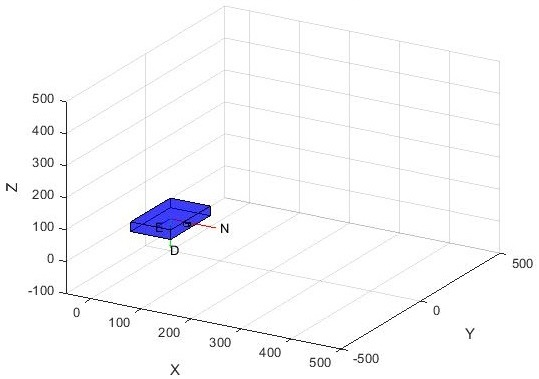
\includegraphics[width=\textwidth]{\IMAGEPATH Data/voxelize0s}
		\caption{Initial (empty) environment}
		\label{fig:scaninit}
	\end{subfigure}
	
	\begin{subfigure}[b]{0.55\textwidth}
		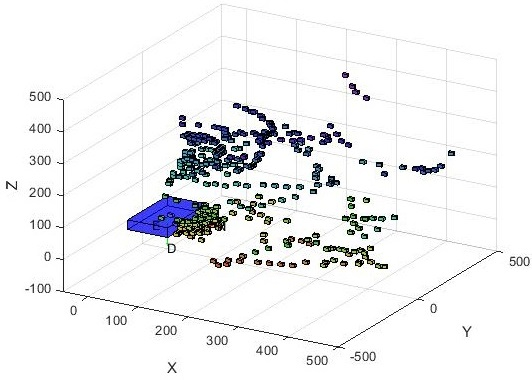
\includegraphics[width=\textwidth]{\IMAGEPATH Data/voxelize10s}
		\caption{10s of data acquisition}
		\label{fig:scanten}
	\end{subfigure}
	
	\begin{subfigure}[b]{0.55\textwidth}
		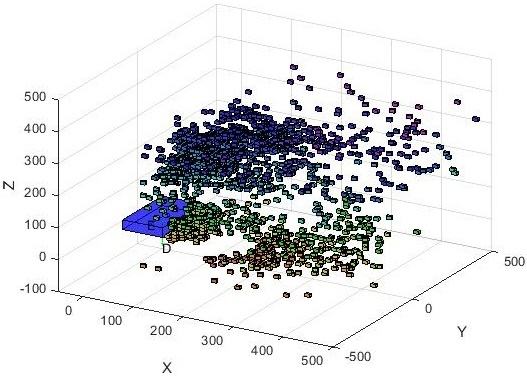
\includegraphics[width=\textwidth]{\IMAGEPATH Data/voxelize60s}
		\caption{60s of data acquisition}
		\label{fig:scanminute}
	\end{subfigure}
	\caption{Scanning the environment with the LiDAR}
	\label{fig:scan}
\end{figure}

\red{
\section{Remaining Sections}
The main argument will begin with a section describing your team's major activities, leading to the fulfillment of the objectives of your project.  A flow chart will provide a useful visual aid.

Introduce the tasks that you were required to complete to satisfy the agreed project scope. Itemise tasks whenever possible to assist cross-referencing with following sections (i.e. your contributions).

Describe the development your ideas and strategies, the conceptual design and research methods used (as applicable), and why they were chosen (your literature review will be of value here).  

Discuss any original contributions including, for example, modifications or extensions of published methods or associated knowledge.  Your team may have made a more humble, but still valuable, contribution, where you customised an existing method for your specific application.  Describe the benefits and, if applicable, deficiencies associated with your contributions.

The criteria against which preferred concepts are identified should be discussed.  This aspect of your report, appropriately sectioned, will make extensive use of pictorial information (figures) and organised information (lists and tables).  

The details of completed analyses and supporting calculations can be included in an Appendix, referred to, as required, from the main body of the report.  Summaries, flow charts identifying methodologies, and sample calculations should be included in the main body of the report.
}

\section{Conclusions and Recommendations}
\subsection{Achievements}
This project set out to develop a prototype UAV with a novel hybrid flight system, capable of competing in the 2016 UAV Challenge - Medical Express. The primary objectives identified in Section \ref{sec:intro} were
\begin{enumerate}[label=\bfseries O\arabic*:] \itemsep-2pt
	\item Register for the 2016 UAV Challenge
	\item Development of a prototype UAV for future teams to build on
	\item Development of autonomous flight controls to achieve \textbf{R1}
	\item Development of a novel hybrid flight system, incorporating both Vertical Take-Off and Landing (VTOL) and Fixed-Wing flight modes, for future teams to build upon to achieve requirements \textbf{R2}, \textbf{R3} and \textbf{R4}
	\item Development of in-flight search and obstacle avoidance mechanisms to be able to achieve \textbf{R5}
\end{enumerate}

Through extensive design and development, \ID have successfully achieved objectives \textbf{O1-O4}, and developed a strong foundation for competing in the 2016 UAV Challenge. Registration for the UAV Challenge was completed in September with the submission of Deliverable \#1, a short technical overview of our proposed aircraft.\\

Testing on the Dragonfly prototype proved that the aircraft was capable of sustained rotor-based flight, successfully achieving flight maneuver \textbf{M1}. The UAV is also equipped with a novel transition system, allowing it to convert between fixed-wing and VTOL flight modes at will, and providing benefits not found on either a purely fixed-wing or rotor-based aircraft. With the addition of the transition system, the prototype has the capability to land in any open terrain without a runway, unlike a regular fixed-wing aircraft, and has the capability to fly long-range or high-endurance missions, unlike a rotor-based aircraft.\\

The UAV is also capable of autonomous flight maneuvers, using a Raspberry Pi to interface with sensors throughout the aircraft, to generate and send flight paths to the PixHawk flight controller. The autonomous flight controls were successfully tested in simulation and on a proxy aircraft, and are ready for testing on the Dragonfly prototype. The software framework that was developed is also readily extensible to add complex flight behaviour not found in commercial UAVs, such as search, obstacle avoidance, and object detection to achieve objective \textbf{O5}.\\

Team \ID have successfully developed a cost-competitive autonomous UAV with hybrid flight, sensing and intelligence capabilities not found on current off-the-shelf products. While the UAV was designed in order to compete in the 2016 UAV Challenge, the novel flight system is cutting-edge research for autonomous aircraft, with applications ranging from emergency response, to delivery and transport, to defence, and far beyond.

\subsection{Further Work}
\red{Path planning\\

Prototype 3\\

Remaining submissions for UAV Challenge\\

\red{Install sensors - can we do this post report?\\}

Electronics architecture - wiring, circuit boards\\}

\subsection{Recommendations}
\red{A recent addition to the flight controller market, the NAVIO+\cite{ref:navio}, is designed for UAVs with vision control applications, and may be better suited for our application.\\
 
Naming of the next prototype ``Mosquito''.\\

Fixed wing automation \& control\\

Tests on battery and prop combo life times\\

Cooling or ventilation system\\

In-flight communications (Rocket M5s)\\

Look at last years winning team

Second Pi\\
}



\red{Confirm that the objectives stated in the Introduction have been met. If the objectives in the Scope of Works document have not been fully met, an argument is required as to why the outcomes do not correspond with those envisaged.

Opportunities for further work, identified through the activities of the current project but outside its scope, should be identified.

This section will summarise your team’s final response to the initial “question, problem or issue”.  A summary of the arguments associated with your outcomes will be provided so that the reader is aware of your reasoning.

Do not include any personal responses to the project (eg. “...we enjoyed working with Joe and learnt a lot from Jen...”).  Write this report as if you are a professional practitioner, representing a research organization or consulting design bureau.

You are encouraged offer details of successful task completion. “Success” can be interpreted in many ways, for example: 
•	Team CP-xxxx contributed “X” to the overall “Y” research program led by Professor “Z”
•	“The client mentor was satisfied with the alternative conceptual designs offered by team CP-xxxx”
•	“The leader of the research division of the collaborating organisation was impressed with the alternative experimental method proposed by team CP-xxxx”
•	“An extensive review of the scientific literature has been completed by team CP-xxxx”
•	“Commercially available solutions were identified and ranked against criteria developed in conjunction with the client”

You can report on the status of your contributions.  For example, within the collaborating “research laboratory”, “research group”, “research initiative”, or “client company”, the final proposals of team CP-xxxx:
•	have been implemented,
•	are under review for later implementation,
•	are awaiting detailed costing, or
•	have provided a range of novel alternative strategies for later consideration.

Do not “apologise”.  Focus only on the positive outcomes of your work.  As an example, it is likely that tasks identified in your Scope of Works but not completed would have required more resources than were available.  Identify important tasks not completed as opportunities for further work within the associated DME laboratory or client organization, and discuss why they are important.  Given the many tasks that you have likely completed, your team now have an excellent knowledge of the requirements of the tasks not completed – briefly outline your expectation of the resources (i.e. personnel expertise, equipment, facilities, finance) needed to complete important tasks.}

\newpage

\printbibliography

\appendix

\newpage

\section{Additional Work}
\label{sec:AppA}
\red{Detailed work completed by the project team not included in the main body (calculations, sketches, details of activities not suited to the main body, e.g. raw data from experiments).}

\subsection{Analysis of 2014 Aircraft}
\label{sec:lastYear}
Research \red{Any references to add here?} suggests that a Y6 configuration, with 3 sets of 2 coaxial motors (2 pairs at the front, 1 at the rear), is the best setup for this task, as shown on the FireFLY6 in Figure \ref{fig:firefly6} above. However, due to its weight and construction, this is not possible on the 2014 model. Instead, it will have to be fitted in quadrotor formation, with four motors and rotors attached under the fuselage, as in Figure \ref{fig:arcturus}. To hover the aircraft (22kg) with 4 (3.5kg) motors equipped with 20 inch (50cm) propellers, in air with density 1.168 kg/m3 would require\\

\begin{tabular}{r c l}
	$P$ & $=$ & $N_{motors} \times v_{air} \times F_{thrust}$\\
	& $=$ & $N_{motors} \times \sqrt{F_{thrust}/(\rho_{air} \times \pi \times r_{prop}^2)} \times F_{thrust}$\\
	& $=$ & $N_{motors} \times F_{thrust}^{3/2}/\sqrt{\rho_{air} \times \pi \times r_{prop}^2}$\\
	& $=$ & $(mg)^{3/2}/\sqrt{N_{motors} \times \rho_{air} \times \pi \times r_{prop}^2}$\\
	& $=$ & $6930W$\\
\end{tabular}
\vspace{6pt}
	
This requirement assumes it is under ideal conditions (100 percent motor and rotor efficiency). It would be incredibly difficult to find a motor with the capabilities required, and at a reasonable price. More significant however is the battery required. Even if the battery weight is neglected, under a 10 cell (37 Volt) load, 200A would be required just to hover. This would be incredibly dangerous and under real conditions it would be much higher. Flight time with the available batteries would be extremely short. On the largest 10 cell batteries available at hobbyking, Zippy Compact 5800mAH, this would only amount to 100 seconds of flight time. The mission would require at least 4 for the VTOL take off and landing procedures alone. This would equate to 736AUD and 5kg of extra weight.\\

In addition to cost and flight time, the modifications necessary to make such a plane would be significantly more difficult, as the supports would need to hold much more weight, and the plane itself is made of wood and not foam. The design of the hybrid craft on the larger plane would have a significant amount of aerodynamic drag and be less efficient. It would look something like the Arcturus, see Figure \ref{fig:arcturus}.\\
	
Last year's project was designed for a very different challenge where VTOL was not required. It was also designed as a multi-platform craft, where the fixed wing was designed for manufacture, something that was not planned in this year's scope. With consideration to all of the above points, it is believed that purchasing a foam model airframe for UAV development was the best course of action for \ID.

\subsection{Stall Speed}
\label{sec:stall}
As lift(N): $L = 1/2\times C_l\times\rho\times A\times V^2$\\\\
Airspeed ($ms^{-1})$:\\
$V= \sqrt{\frac{2\times L}{C_l\times \rho \times A}}$\\
$V = 12.66ms^{-1} = 45.5kmh^{-1}$\\\\
Where:\\
Required lift: $L = 4kg \times ms^{-2} = 39.24N$\\
Air density at sea level: $\rho = 1.225 kgm^{-1}$\\
Area of Skywalker Wings: $A = 0.8m^2$\\
Worst case coefficient of lift when attempting to climb (see Figure \ref{fig:lift})  
: $C_l = 0.5$
\\\\
\begin{figure}[!h]
	\centering
	\includegraphics[width=300pt]{\IMAGEPATH lift_coeff}
	\caption{Skywalker X8 lift coefficient (green) vs angle of attack}
	\label{fig:lift}
\end{figure}

\todomessage{reference the graph, and order it better}

\subsection{Gyroscopic Effects}
\label{sec:gyro}
Angular momentum of propellers: $H = I\omega$\\
Maximum motor speed $\omega = 800\times16.8\times\frac{2\pi}{60} = 1407.45rads^{-1}$\\
Prop Inertia $I = \frac{1}{12}\times M(L^2+B^2) = 1.16\times10^{-4}kgm^2$ (Overestimate, as it assumes equally distributed mass, and constant width)\\\\

\begin{figure}[!h]
	\includegraphics[width=100pt]{\IMAGEPATH angular_momentum}
\end{figure}

Using a small angle approximation $\Delta H = \omega_p \times\Delta t \times I \times \omega$\\ 
$\omega_p$ = Maximum servo rotation speed (procession) = $frac{60^o}{0.11s} = 9.52rads^{-1}$\\
$\frac{dH}{dt} = \omega_p \times I \times \omega = M = 1.55Nm$\\\\

\begin{figure}[!h]
	\includegraphics[width=100pt]{\IMAGEPATH moments}
\end{figure}

 Counter-rotating propellers stop the drone from yawing (and possibly spinning out of control on transition), as the moments act in opposite directions. They also act to make gyroscopic forces on the servo negligible due to them counteracting each other in a twist motion when the drone rolls fast, rather than placing a moment on the servos.\\\\
Max moment in the centre of the front shaft is $2M = 3.1Nm$. If this is less than the moment on the front bar at hover ($2/3$ $\times M \times d$) then the shaft should be capable of withstanding the gyroscopic effects, as the moment created is less than that created by the weight of the plane at hover.\\

$3.1Nm < 9.156Nm$, therefore It should be able to withstand the gyroscopic moments easilly.

\subsection{eCalc Modelling}
\label{sec:ecalc}
\begin{figure}[H]
	\centering
	\includegraphics[width=400pt]{\IMAGEPATH /Ecalc/eCalc1}
	\caption{Fixed-wing performance, 11 inch props}
\end{figure}
\begin{figure}[H]
	\centering
	\includegraphics[width=400pt]{\IMAGEPATH /Ecalc/eCalc2}
	\caption{VTOL performance, 11 inch props}
\end{figure}
\begin{figure}[H]
	\centering
	\includegraphics[width=400pt]{\IMAGEPATH /Ecalc/eCalc3}
	\caption{Fixed-wing performance, 12 inch props}
	\label{fig:fixed}
\end{figure}
\begin{figure}[H]
	\centering
	\includegraphics[width=400pt]{\IMAGEPATH /Ecalc/eCalc4}
	\caption{VTOL performance, 12 inch props}
	\label{fig:vtol}
\end{figure}
\begin{figure}[H]
	\centering
	\includegraphics[width=400pt]{\IMAGEPATH /Ecalc/eCalc7}
	\caption{Fixed-wing performance, 12 inch props, 3 batteries}
\end{figure}
\begin{figure}[H]
	\centering
	\includegraphics[width=400pt]{\IMAGEPATH /Ecalc/eCalc8}
	\caption{VTOL performance, 12 inch props, 3 batteries}
\end{figure}

\newpage

\section{Project Administration}
Management and administration information:
•	Gantt chart (schedule) – Include important issues associated with task duration prediction – presented in your “Progress Reports”.
•	Cumulative hours spent on project – individual and/or team based, project diaries, meeting minutes or summaries (i.e. useful outcomes from each meeting).  Each meeting will require a numeric identifier if you are to reference expert opinion in the main body of your report (eg. “Section A.2.3”).
•	Individual or team based project diary.
•	Copy of your final Scope of Works.


\end{document}
